\documentclass[11pt]{article}\usepackage[]{graphicx}\usepackage[]{color}
% maxwidth is the original width if it is less than linewidth
% otherwise use linewidth (to make sure the graphics do not exceed the margin)
\makeatletter
\def\maxwidth{ %
  \ifdim\Gin@nat@width>\linewidth
    \linewidth
  \else
    \Gin@nat@width
  \fi
}
\makeatother

\definecolor{fgcolor}{rgb}{0.345, 0.345, 0.345}
\newcommand{\hlnum}[1]{\textcolor[rgb]{0.686,0.059,0.569}{#1}}%
\newcommand{\hlstr}[1]{\textcolor[rgb]{0.192,0.494,0.8}{#1}}%
\newcommand{\hlcom}[1]{\textcolor[rgb]{0.678,0.584,0.686}{\textit{#1}}}%
\newcommand{\hlopt}[1]{\textcolor[rgb]{0,0,0}{#1}}%
\newcommand{\hlstd}[1]{\textcolor[rgb]{0.345,0.345,0.345}{#1}}%
\newcommand{\hlkwa}[1]{\textcolor[rgb]{0.161,0.373,0.58}{\textbf{#1}}}%
\newcommand{\hlkwb}[1]{\textcolor[rgb]{0.69,0.353,0.396}{#1}}%
\newcommand{\hlkwc}[1]{\textcolor[rgb]{0.333,0.667,0.333}{#1}}%
\newcommand{\hlkwd}[1]{\textcolor[rgb]{0.737,0.353,0.396}{\textbf{#1}}}%
\let\hlipl\hlkwb

\usepackage{framed}
\makeatletter
\newenvironment{kframe}{%
 \def\at@end@of@kframe{}%
 \ifinner\ifhmode%
  \def\at@end@of@kframe{\end{minipage}}%
  \begin{minipage}{\columnwidth}%
 \fi\fi%
 \def\FrameCommand##1{\hskip\@totalleftmargin \hskip-\fboxsep
 \colorbox{shadecolor}{##1}\hskip-\fboxsep
     % There is no \\@totalrightmargin, so:
     \hskip-\linewidth \hskip-\@totalleftmargin \hskip\columnwidth}%
 \MakeFramed {\advance\hsize-\width
   \@totalleftmargin\z@ \linewidth\hsize
   \@setminipage}}%
 {\par\unskip\endMakeFramed%
 \at@end@of@kframe}
\makeatother

\definecolor{shadecolor}{rgb}{.97, .97, .97}
\definecolor{messagecolor}{rgb}{0, 0, 0}
\definecolor{warningcolor}{rgb}{1, 0, 1}
\definecolor{errorcolor}{rgb}{1, 0, 0}
\newenvironment{knitrout}{}{} % an empty environment to be redefined in TeX

\usepackage{alltt}

\usepackage{rotating}
\usepackage{graphics}
\usepackage{latexsym}
\usepackage{color}
\usepackage{listings}
\usepackage{wrapfig}
\usepackage{float}
\usepackage[belowskip=-15pt,aboveskip=0pt]{caption}

\setlength\topmargin{-.56in}
\setlength\evensidemargin{0in}
\setlength\oddsidemargin{0in}
\setlength\textwidth{6.49in}
\setlength\textheight{8.6in}
\setlength{\intextsep}{10pt plus 1pt minus 4pt}

\definecolor{codegreen}{rgb}{0,0.6,0}
\definecolor{codegray}{rgb}{0.5,0.5,0.5}
\definecolor{codepurple}{rgb}{0.58,0,0.82}
\definecolor{backcolour}{rgb}{0.95,0.95,0.92}
\lstdefinestyle{mystyle}{
	backgroundcolor=\color{backcolour},   
	commentstyle=\color{codegreen},
	keywordstyle=\color{magenta},
	numberstyle=\tiny\color{codegray},
	stringstyle=\color{codepurple},
	basicstyle=\footnotesize,
	breakatwhitespace=false,         
	breaklines=true,                 
	captionpos=b,                    
	keepspaces=true,                 
	numbers=left,                    
	numbersep=5pt,                  
	showspaces=false,                
	showstringspaces=false,
	showtabs=false,                  
	tabsize=2
}
\lstset{style=mystyle}

\pagestyle{headings}

\title{Penetration Rates for Prostate Cancer\vspace{-5ex}} 
\date{November 12, 2020\vspace{-5ex}}
\IfFileExists{upquote.sty}{\usepackage{upquote}}{}
\begin{document} 
\maketitle
\hfill \break










\noindent\textbf{\underline{Executive Summary}}: 
\hfill \break

\noindent\textbf{\underline{Introduction}}: 
\hfill \break

\noindent\textbf{\underline{Methods}}:    
\hfill \break

\noindent\textbf{\underline{Exploratory Data Analysis}}: 
\hfill \break

\begin{figure}[h!] 
\begin{center}

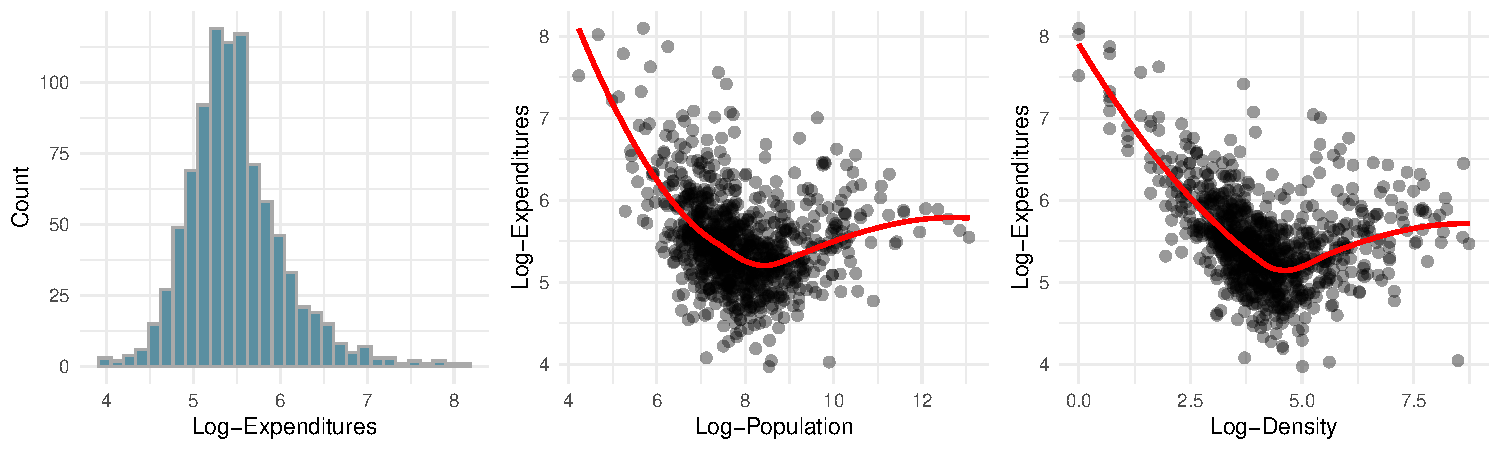
\includegraphics[width=\maxwidth]{figure/unnamed-chunk-1-1} 

\caption{}
\label{explore1}
\end{center} 
\end{figure}


\begin{figure}[h!] 
\begin{center}

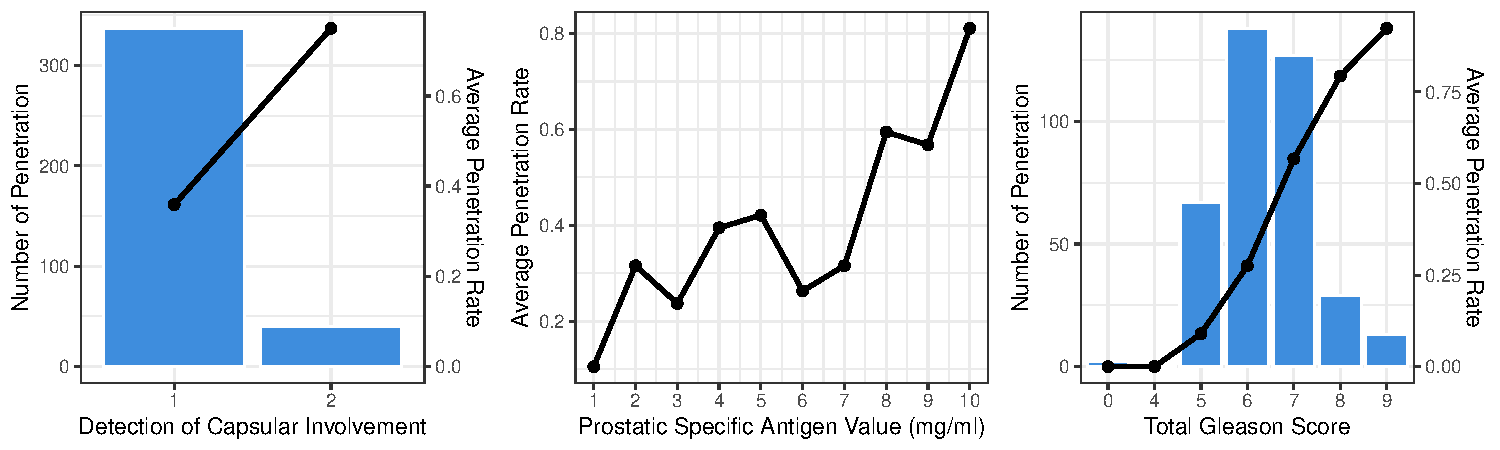
\includegraphics[width=\maxwidth]{figure/unnamed-chunk-2-1} 

\caption{}
\label{explore2}
\end{center} 
\end{figure}




\noindent\textbf{\underline{Model Fitting/Inferences}}: 
\hfill \break







\begin{center}
% latex table generated in R 3.6.2 by xtable 1.8-4 package
% Sat Nov 07 17:54:24 2020
\begin{table}[ht]
\centering
\begin{tabular}{lrrrrrrr}
  \hline
term & estimate & std.error & statistic & p.value & OR & 2.5 \% & 97.5 \% \\ 
  \hline
(Intercept) & -7.254 & 1.296 & -5.595 & 0.000 & 0.001 & 0.000 & 0.008 \\ 
  dpros2 & 0.822 & 0.461 & 1.785 & 0.074 & 2.276 & 0.944 & 5.835 \\ 
  dpros3 & 1.306 & 0.483 & 2.700 & 0.007 & 3.689 & 1.466 & 9.892 \\ 
  dpros4 & 1.280 & 0.577 & 2.220 & 0.026 & 3.598 & 1.176 & 11.452 \\ 
  psa & 0.041 & 0.015 & 2.760 & 0.006 & 1.042 & 1.015 & 1.075 \\ 
  gleason & 0.846 & 0.200 & 4.231 & 0.000 & 2.331 & 1.599 & 3.514 \\ 
   \hline
\end{tabular}
\caption{Summary regression of final model} 
\label{reg_summary_final}
\end{table}

\end{center}


\begin{figure}[h!] 
\begin{center}

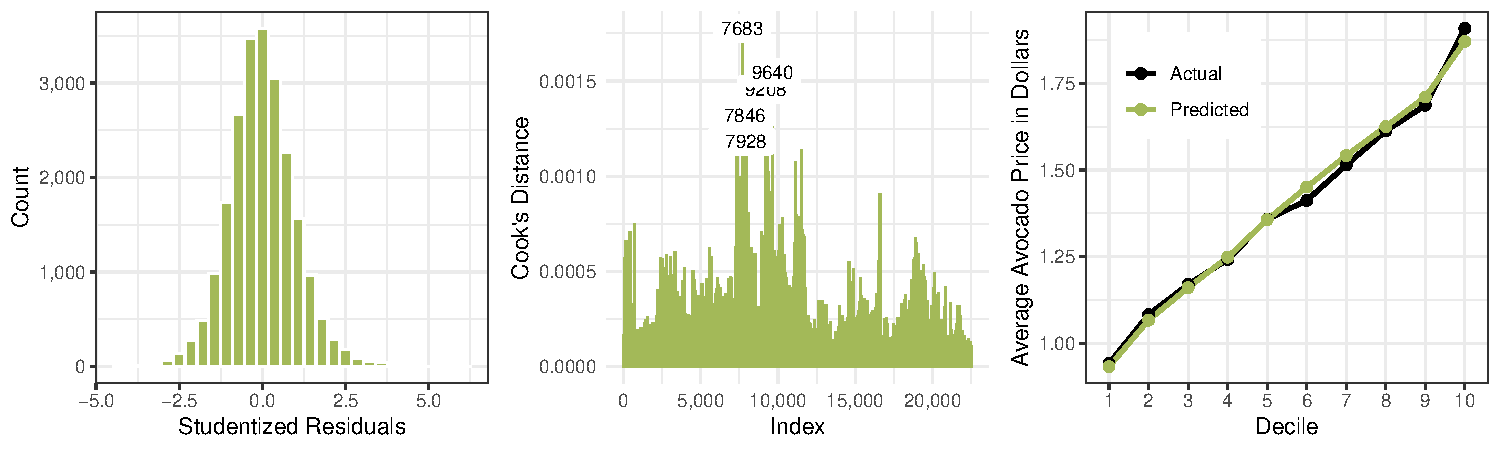
\includegraphics[width=\maxwidth]{figure/unnamed-chunk-4-1} 

\caption{}
\label{model_plot_1}
\end{center} 
\end{figure}


\begin{figure}[h!] 
\begin{center}

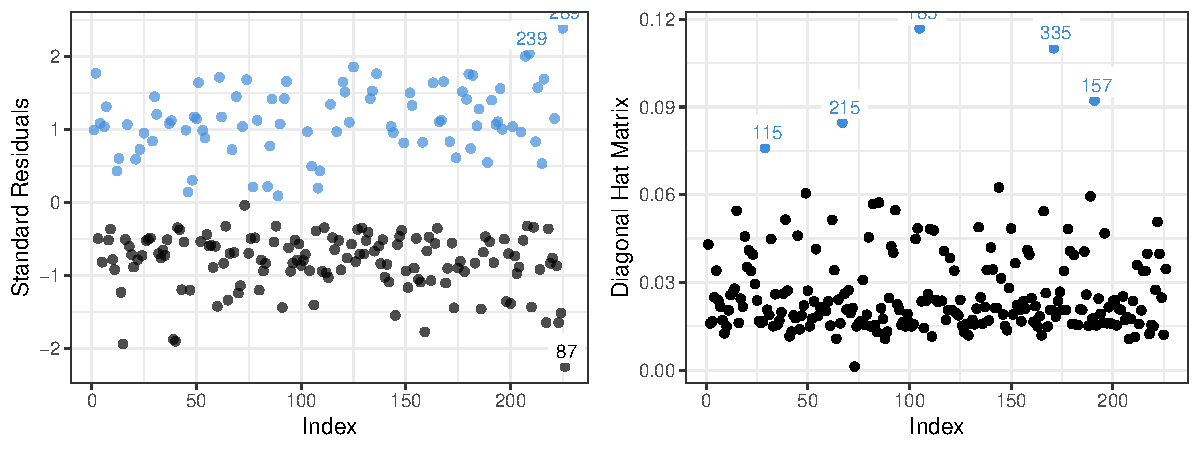
\includegraphics[width=\maxwidth]{figure/unnamed-chunk-5-1} 

\caption{}
\label{model_plot_1}
\end{center} 
\end{figure}


\noindent\textbf{\underline{Conclusion}}: 
\hfill \break

\clearpage
\newpage
\noindent \Large{{\bf Appendix A: Supplemental Tables}}

\begin{center}

% Table created by stargazer v.5.2.2 by Marek Hlavac, Harvard University. E-mail: hlavac at fas.harvard.edu
% Date and time: Sat, Nov 07, 2020 - 5:54:25 PM
\begin{table}[H] \centering 
  \caption{Summary Statistics for all numerical independent features} 
  \label{descrips} 
\begin{tabular}{@{\extracolsep{5pt}}lccccccc} 
\\[-1.8ex]\hline 
\hline \\[-1.8ex] 
Statistic & \multicolumn{1}{c}{N} & \multicolumn{1}{c}{Mean} & \multicolumn{1}{c}{St. Dev.} & \multicolumn{1}{c}{Min} & \multicolumn{1}{c}{Pctl(25)} & \multicolumn{1}{c}{Pctl(75)} & \multicolumn{1}{c}{Max} \\ 
\hline \\[-1.8ex] 
capsule & 377 & 0.401 & 0.491 & 0 & 0 & 1 & 1 \\ 
age & 377 & 66.066 & 6.425 & 47 & 62 & 71 & 79 \\ 
psa & 377 & 15.256 & 19.869 & 0.300 & 5.000 & 16.800 & 139.700 \\ 
gleason & 377 & 6.379 & 1.092 & 0 & 6 & 7 & 9 \\ 
psa\_bins & 377 & 5.472 & 2.869 & 1 & 3 & 8 & 10 \\ 
\hline \\[-1.8ex] 
\end{tabular} 
\end{table} 

\end{center} 

\begin{center}
% latex table generated in R 3.6.2 by xtable 1.8-4 package
% Sat Nov 07 17:54:25 2020
\begin{table}[ht]
\centering
\begin{tabular}{rrrrlrr}
  \hline
 & random\_partition & nrow\_train & nrow\_test & features & AIC & auc \\ 
  \hline
1 & 0.900 &  339 &   38 & dpros,psa,gleason,dcaps & 298.077 & 0.822 \\ 
  2 & 0.800 &  301 &   76 & dpros,psa,gleason,dcaps & 278.940 & 0.820 \\ 
  3 & 0.600 &  226 &  151 & dpros,psa,gleason & 241.799 & 0.819 \\ 
  4 & 0.700 &  263 &  114 & dpros,psa,gleason & 260.832 & 0.818 \\ 
  5 & 0.600 &  226 &  151 & dpros,psa,gleason,dcaps & 240.567 & 0.818 \\ 
  6 & 0.700 &  263 &  114 & dpros,psa,gleason,dcaps & 258.675 & 0.815 \\ 
  7 & 0.900 &  339 &   38 & dpros,psa,gleason & 297.050 & 0.812 \\ 
  8 & 0.800 &  301 &   76 & dpros,psa,gleason & 277.654 & 0.809 \\ 
  9 & 0.600 &  226 &  151 & psa,gleason,dcaps & 251.167 & 0.805 \\ 
  10 & 0.900 &  339 &   38 & dpros,gleason & 301.355 & 0.805 \\ 
   \hline
\end{tabular}
\caption{} 
\label{reg_bootstrap}
\end{table}

\end{center}

\begin{center}
% latex table generated in R 3.6.2 by xtable 1.8-4 package
% Sat Nov 07 17:54:25 2020
\begin{table}[ht]
\centering
\begin{tabular}{rrrrr}
  \hline
 & Estimate & Std. Error & z value & Pr($>$$|$z$|$) \\ 
  \hline
(Intercept) & -9.7465 & 3.8714 & -2.52 & 0.0118 \\ 
  dpros2 & 1.7503 & 4.1518 & 0.42 & 0.6733 \\ 
  dpros3 & 2.9024 & 4.2654 & 0.68 & 0.4962 \\ 
  dpros4 & 4.8459 & 4.7046 & 1.03 & 0.3030 \\ 
  psa & 0.2090 & 0.1227 & 1.70 & 0.0886 \\ 
  gleason & 1.0748 & 0.6161 & 1.74 & 0.0811 \\ 
  dpros2:psa & -0.0986 & 0.0638 & -1.55 & 0.1221 \\ 
  dpros3:psa & -0.1225 & 0.0801 & -1.53 & 0.1260 \\ 
  dpros4:psa & -0.0601 & 0.0699 & -0.86 & 0.3902 \\ 
  dpros2:gleason & 0.0468 & 0.6584 & 0.07 & 0.9434 \\ 
  dpros3:gleason & -0.0354 & 0.6803 & -0.05 & 0.9585 \\ 
  dpros4:gleason & -0.4452 & 0.7431 & -0.60 & 0.5491 \\ 
  psa:gleason & -0.0130 & 0.0168 & -0.77 & 0.4396 \\ 
   \hline
\end{tabular}
\caption{} 
\label{reg_summary_int}
\end{table}

\end{center}

\begin{center}
% latex table generated in R 3.6.2 by xtable 1.8-4 package
% Sat Nov 07 17:54:25 2020
\begin{table}[ht]
\centering
\begin{tabular}{rrlrrl}
  \hline
 & capsule & dpros & psa & gleason & rownames \\ 
  \hline
1 &   0 & 2 & 51.20 &   7 & 4 \\ 
  2 &   0 & 4 & 31.90 &   7 & 7 \\ 
  3 &   0 & 4 & 17.10 &   9 & 87 \\ 
  4 &   1 & 4 & 45.30 &   6 & 115 \\ 
  5 &   0 & 4 & 25.20 &   7 & 121 \\ 
  6 &   1 & 1 & 44.40 &   6 & 157 \\ 
  7 &   1 & 1 & 85.40 &   7 & 185 \\ 
  8 &   1 & 3 & 17.70 &   5 & 196 \\ 
  9 &   1 & 4 & 53.90 &   6 & 215 \\ 
  10 &   1 & 1 & 6.70 &   6 & 239 \\ 
  11 &   0 & 4 & 25.10 &   7 & 254 \\ 
  12 &   1 & 4 & 18.70 &   5 & 267 \\ 
  13 &   1 & 1 & 8.90 &   6 & 272 \\ 
  14 &   1 & 1 & 6.80 &   5 & 289 \\ 
  15 &   0 & 3 & 18.10 &   8 & 307 \\ 
  16 &   1 & 2 & 58.00 &   6 & 335 \\ 
  17 &   0 & 2 & 48.00 &   7 & 365 \\ 
   \hline
\end{tabular}
\caption{} 
\label{outlier_obs}
\end{table}

\end{center}


\clearpage
\newpage
\noindent \Large{{\bf Appendix B: R Code}}
\lstinputlisting[language=R, caption = Appendix of Code]{R/dar2-codes.R}


\end{document}






